\documentclass[]{article}

\author{Rushi Shah}
\date{\today}
\title{Automating Code and Data Migration \\ After Schema Refactorings}


\usepackage{setspace}
\doublespacing
% or:
% \onehalfspacing

\usepackage{amsmath}
\usepackage{amsthm}
\usepackage{amssymb}
\usepackage{mathtools}
\usepackage{graphicx}
\usepackage{hyperref}
\usepackage{algorithm}
\usepackage{algpseudocode}
\usepackage{listings}

\usepackage{adjustbox}
\usepackage{algorithm}
\usepackage{amsmath}
\usepackage{amssymb}
\usepackage{bbm, dsfont}
\usepackage{stmaryrd}
\usepackage{url}
\usepackage{listings}
\usepackage{xcolor}
\usepackage{graphicx}
\usepackage{wrapfig}
\usepackage{caption}
\usepackage{subcaption}
\usepackage{mathrsfs}
\usepackage{esvect}
\usepackage{xspace}
\usepackage{array, multirow}
\usepackage{rotating, makecell}
\usepackage{enumitem}
\usepackage{tikz} \usetikzlibrary{patterns}
\usepackage{pgfplots}
\usepackage{filecontents}
\usepackage{comment}
\usepackage{balance}

% \pgfplotsset{compat=1.12}

\usepackage{graphicx}
\graphicspath{ {./resources/} }

\usepackage[margin=1.5in]{geometry}

\newcommand{\integers}{\mathbb{Z}}
\newcommand{\naturals}{\mathbb{N}}
\newcommand{\reals}{\mathbb{R}}
\newcommand{\complexes}{\mathbb{C}}
\newcommand{\rationals}{\mathbb{Q}}
\newcommand{\inv}{^{-1}}
\newcommand{\bits}{\{0, 1\}}
\DeclarePairedDelimiter\floor{\lfloor}{\rfloor}

\begin{document}
    
\begin{titlepage}
    \begin{center}
        \vspace*{1cm}
            
        \huge
        \textbf{Automating Code and Data Migration After Schema Refactorings \\}
        \vspace{0.5cm}
        \Large
        Rushi Shah


        \vspace{1.5cm}
        \large
        \textit{A thesis presented for the Turing Scholar honors distinction.}
            
        % \vspace{1.5cm}
            
        \vfill
            
        % A thesis presented for Turing Scholar honors distinction. 
            
            
        
\includegraphics[width=.4\textwidth]{texas_shield}

        \vfill
            
        \Large
        Department of Computer Science\\
        University of Texas at Austin\\
        \today
            
    \end{center}
\end{titlepage}

    \maketitle

    \section{Abstract}

        This thesis describes two techniques for automating web application developer tasks created when the application's underlying database schema is refactored. These schemas are generally refactored to improve performance or maintainability, but doing so creates two programmer tasks: code migration and data migration. My research with the UT Program Analysis (UToPiA) research group automates both tasks for developers. Our first research result for code migration, called Migrator, appeared at Programming Languages Design and Implementation 2019 \cite{pldi19}. Our second research result, called Dynamite, will appear at the Conference on Very Large Databases 2020 \cite{vldb20}.

        % maybe talk about how the automation comes from program synthesis

    % \section{Introduction}

    % Something like this: "Programmers face difficulties when writing safe and correct programs in a variety of domains. One solution to these difficulties is program synthesis. Synthesis tools aim to generate code from some higher level specification. These specifications are usually much easier for programmers to supply than the actual code. For example, the user might give one or more input-output examples of what their desired program should do."

    % With these insights in mind, we present two contributions in this report. T

    % Our first contribution aims to

    % Our second contribution aims to 

    \section{Code Migration with Migrator}

        \subsection{Introduction}

            Code migration refers to the program changes that need to be made to a web application to preserve functionality in the face of a new database schema. Database schemas are often updated for performance or maintainability reasons, but the corresponding program changes are tedious and error prone when done by hand. In contrast, we implemented a fully automated solution called Migrator that takes as input the old program, old schema, and new schema, and synthesizes a new program that is verifiably equivalent to the old program. We were able to successfully synthesize new programs in ten examples collected from textbooks on the subject and ten real world Ruby on Rails applications collected from GitHub. My role in this project was primarily to evaluate our tool against the previous state of the art, so I re-implemented our approach in a popular synthesis framework called Sketch. My experiments showed that Sketch failed to synthesize a majority of the benchmarks, and furthermore showed that our tool works 1,700 times faster on the benchmarks Sketch actually completes.

        \subsection{Motivating Example}

            Consider the following motivating example, which contains the ID, name, and picture for both ``Instructors'' and ``TAs''. Originally, the database schema may have contained separate tables for each:
             
            \begin{verbatim}
                Instructor(InstrId, InstrName, InstrPic)
                TA(TaId, TaName, TaPic)     
            \end{verbatim}
            
            Then an instructor could be added with the following parameterized operation:

            \begin{verbatim}
                update addInstructor(id, name, pic) 
                    INSERT INTO Instructor VALUES (id, name, pic)
            \end{verbatim}

            However, since accessing a table with large images can be innefficient, perhaps the developers updated the schema to pull out the images into a seperate table that is linked with foreign keys:
            
            \begin{verbatim}
                Instructor(InstrId, InstrName, PictureId)
                TA(TaId, TaName, PictureId) 
                Picture(PictureId, Picture) 
            \end{verbatim}

            Then the program to add a new instructor would need to be edited as follows:
            
            \begin{verbatim}
                update addInstructor(id, name, pic) 
                    INSERT INTO Instructor VALUES (id, name, UID0)
                    INSERT INTO Picture VALUES (UID0, pic)
            \end{verbatim}

            Similar changes would need to be made for each possible relational operation (adding, updating, selecting, etc.) for each table (Instructor, TA, etc.). Our tool automates this process. 


        \subsection{Migrator}

            % high level intro

            Given an existing database program $P$ that operates over source schema $S$ and a new target schema $S'$ that $P$ should be migrated to, our method automatically synthesizes a new database program $P'$ over the new schema $S'$ such that $P$ and $P'$ are semantically equivalent. This ensures that no desirable behaviors of the program are lost and no unwanted behaviors are introduced in the process.



            \subsubsection{Synthesis Methodology}

                \begin{figure*}[]
                    \centering
                    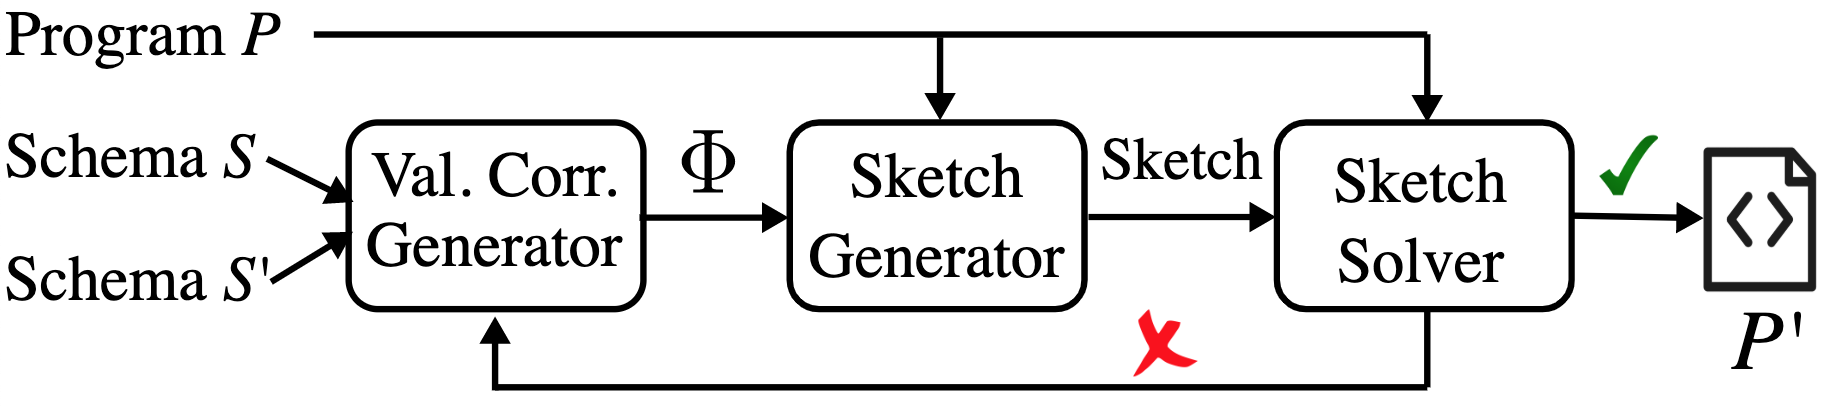
\includegraphics[width=.7\textwidth]{migrator_methodology}
                    \caption{Migrator methodology.}
                    \label{fig:migrator_methodology}
                \end{figure*}

                Our methodology for code migration is illustrated schematically in Figure~\ref{fig:migrator_methodology}. We first generate a \textit{value correspondence} that relates how the values in $S'$ can be obtained from the values in $S$. This value correspondence is used to enumerate the space of possible candidate programs in something called a \textit{program sketch}. This program sketch is then completed using our notion of \textit{minimum failing inputs (MFIs)} to dramatically prune the search space. If our completed sketch $P'$ is semantically equivalent to the desired program $P$, we are done. Otherwise, a new value correspondence is considered and the process repeats. 
            
            \subsubsection{Evaluation against Sketch}

                \begin{figure*}[!t]
                    \centering
                    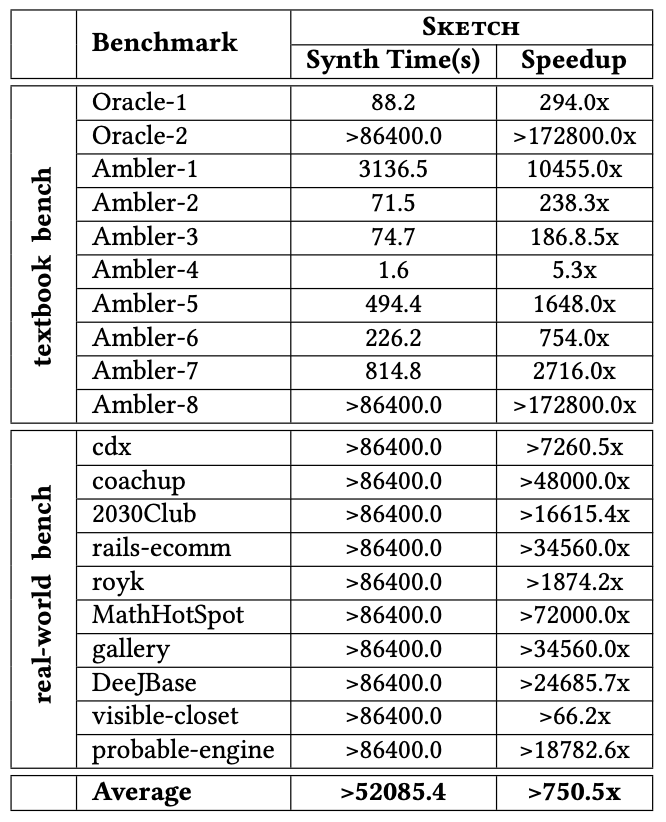
\includegraphics[width=.6\textwidth]{migrator_sketch_results}
                    \caption{Migrator comparison with Sketch.}
                    \label{fig:migrator_sketch_results}
                \end{figure*}

                To evaluate the proposed idea, we use Migrator to automatically migrate 20 database programs to a new schema. All 20 programs in our benchmark set are taken from prior work \cite{wang2017verifying} for verifying equivalence between database programs. Specifically, half of these benchmarks are adapted from textbooks and oline tutorials, and the remaining half are manually extracted from real-world web applications on Github. 

                We evaluated the effectiveness of our MFI approach against the state of the art, namely a  ``Counter-Example Guided Inductive Synthesis (CEGIS)'' approach. To do so, we reimplemented our approach in Sketch, a popular CEGIS tool \cite{sketch}. Sketch uses bounded model checking to automatically complete program sketches. 

                We implemented the semantics of SQL in Sketch by encoding each SQL statement as a C function. Specifically, our Sketch encoding models each database table as an array or arrays, with the nested array representing a tuple, and we model each SQL operation as a function that reads and updates the array as appropriate. The results of this experiment are summarized in Figure~\ref{fig:migrator_sketch_results}. The main observation is that Sketch times out on all real-world benchmarks from Github as well as two textbook examples, namely Oracle-2 and Ambler-8. For all other benchmarks, Migrator is significantly faster than Sketch, with speed-ups ranging between 5.3x to 10455.0x in terms of synthesis time. We believe this experiment demonstrates the advantage of our proposed sketch completion algorithm compared to the standard CEGIS approach implemented in Sketch. 

                % my main contribution


    \section{Data Migration with Dynamite}

        \subsection{Introduction}

            Data migration refers to bringing existing data from the old database to the new database in a way that respects the schema change. Database schemas are often updated for performance or maintainability reasons, but the existing data in the database must be correspondingly updated. Prior work has addressed this goal in restricted formats, for example schema refactorings within one database format (relational format to relational format) or across specific formats (document format to relational format only). But our work, called Dynamite, frames the generalized version of the problem as a Datalog program synthesis problem. 

            Using the internal representation we developed, we can infer a schema mapping between database schemas regardless of what format the source and target databases are in. In particular, we consider document formats like JSON or XML, relational formats like SQL, and graph formats like neo4j. This generality substantially expands the usability of Dynamite to a greater variety of users over the current state-of-the-art, which we demonstrated by migrating real-world databases like IMDB and DBLP across all formats in a matter of minutes.

            My role in this data migration project focused on executing the actual database migrations given the value correspondence from the synthesized Datalog program. To do so, I wrote XML and JSON parsers robust to real-world files that are tens of gigabytes large, and wrote scalable transformers to turn the output of the Datalog program (a CSV file of data) into the final expected format (relational database, graph database, or document database format). Secondly, I was responsible for conducting the experiments with our tool to collect our empirical results. This responsibility included preparing the server for the experiments, preprocessing the benchmarks to remove special characters from the source databases, writing the test for the end-to-end system, conducting the experiments, debugging any errors caused, and compiling the results for their presentation in the paper. 

        \subsection{Motivating Example}

            Consider the following motivating example, in which a relational database called ``Parent'' stores the name of the adult and the name of their kid. The schema and database instance may look like this:

            \begin{verbatim}
                Parent(adult, kid)
                rahil, arjun
                arjun, divya
                arjun, bhavin
                [...]
            \end{verbatim}

            And perhaps, for maintainability reasons, the developers decide to store the same data as a ``Child'' relationship, instead of a ``Parent'' one. The target schema, in this case, would be \texttt{Child(kid, adult)}. As an example on one row in the table, they want to transform the table as follows:

            \begin{verbatim}
                Parent(rahil, arjun) -> Child(arjun, rahil)
            \end{verbatim}

            Our tool will take this source schema, source instance, target schema, and input/output example to automatically output the following target instance:

            \begin{verbatim}
                Child(kid, adult)
                arjun, rahil
                divya, arjun
                bhavin, arjun
                [...]
            \end{verbatim}

        \subsection{Dynamite}

            Our method expresses the correspondence between the source and target schemas as a Datalog program. Then, given an input-output example $(I, O)$, finding a schema mapping between the schemas boils down to inferring a Datalog program $P$ such that $(I, O)$ is a model of $P$. Because a Datalog program is executable, we automate the data migration task by simply executing the synthesized program $P$ on the source instance to output the target instance. 

            \subsubsection{Datalog}

                \begin{figure*}[]
                    \centering
                    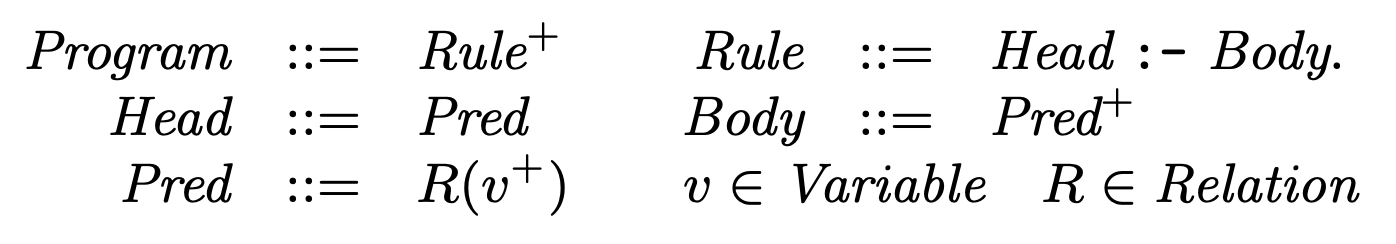
\includegraphics[width=.7\textwidth]{datalog_syntax}
                    \caption{Syntax of Datalog programs.}
                    \label{fig:datalog_syntax}
                \end{figure*}

                For background, Datalog is a declarative programming language. As shown in Figure~\ref{fig:datalog_syntax}, a Datalog program consists of a list of rules, where each rule is of the form $H :- B$. Here, $H$ is referred as the head and $B$ is the body. The head $H$ is a single relation of the form $R(v_1, \ldots, v_n)$, and the body $B$ is a collection of predicates $B_1, B_2, \ldots, B_n$. Predicates that appear only in the body are known as extensional relations and correspond to known facts. Predicates that appear in the head are called intensional relations and correspond to the output of the Datalog program. 

                In our context, we will try to synthesize a Datalog program that represents the relationship between the source database and the target database. Database entries in the source database will correspond to facts in the program (extensional relations). We determine which of these facts combine to create facts in the target database (intensional relations). The relationship between these extensional and intensional relationships (source and target databases, respectively) are captured by the Datalog program, which can then be executed on the source instance. 

            \subsubsection{Synthesis Methodology}

                \begin{figure*}[]
                    \centering
                    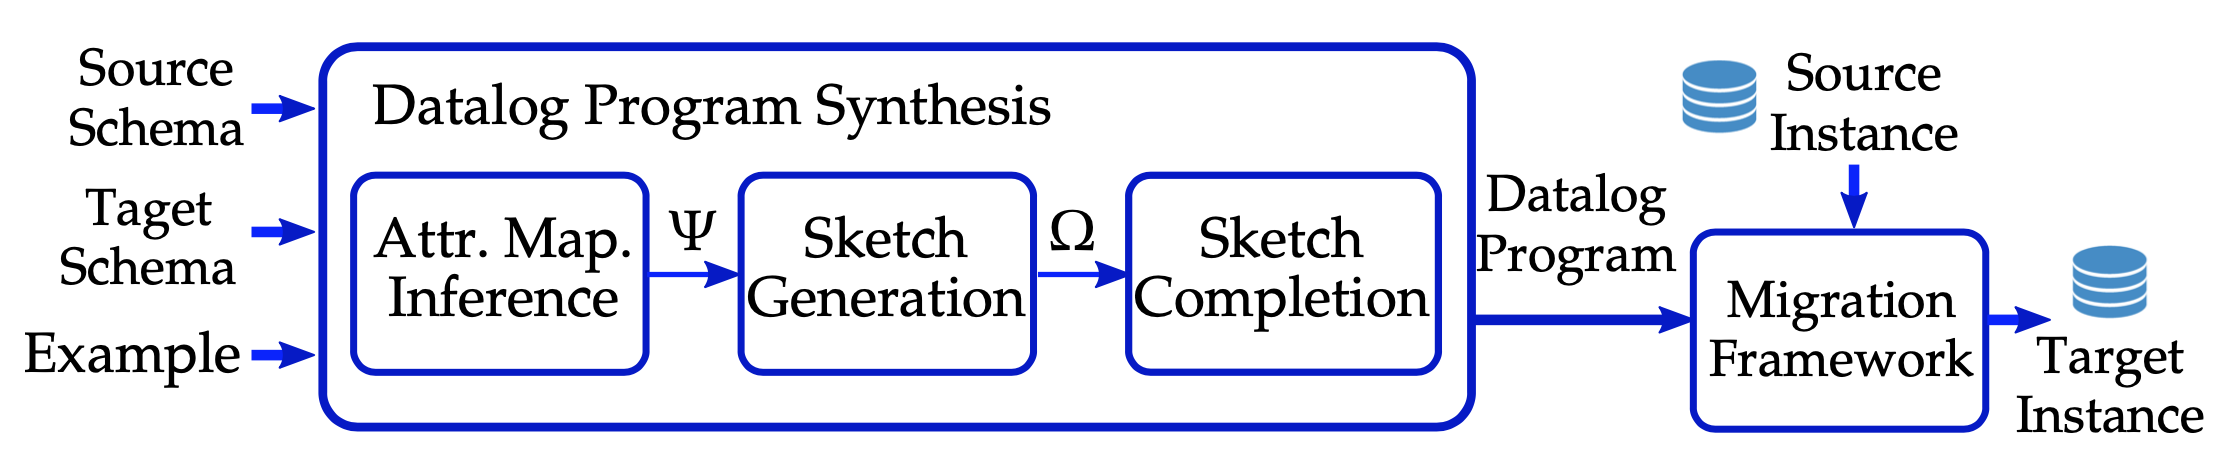
\includegraphics[width=.7\textwidth]{dynamite_workflow}
                    \caption{Schematic workflow of Dynamite.}
                    \label{fig:dynamite_workflow}
                \end{figure*}

                As shown in Figure~\ref{fig:dynamite_workflow}, our approach has three primary steps. We first infer an attribute mapping from each attribute in the source to the set of attributes in the target it could correspond to. We use this attribute mapping to express the search space of all possible schema mappings as a Datalog program sketch. This program sketch is then completed using our notion of \textit{minimum distinguishing projections (MDPs)} to dramatically prune the search space and arrive at the correct Datalog program. This program can be executed on the source instance to efficiently construct the target instance. 

            \subsubsection{Migration Framework}

                % my main contribution

                We have implemented the proposed technique as a new tool called Dynamite. Internally, Dynamite uses the Z3 solver ~\cite{z3-tacas08} for answering SMT queries and leverages the Souffle framework~\cite{souffle-cav16} for evaluating Datalog programs. 

                Dynamite builds the target database instance from the output facts of the synthesized Datalog program as described previously. However, Dynamite performs one optimization to make large-scale data migration practical: We leverage MongoDB~\cite{mongodb-web} to build indices on attributes that connect records to their parents. This strategy allows Dynamite to quickly look up the children of a given record and makes the construction of the target database more efficient. 
            
            \subsubsection{Evaluation}

                \begin{table}
                    \centering
                    \small
                    \begin{tabular}{|c|c|l|}
                    \hline
                    \textbf{Name} & \textbf{Size} & \textbf{Description} \\
                    \hline
                    Yelp & 4.7GB & Business and reviews from Yelp \\
                    \hline
                    IMDB & 6.3GB & Movie and crew info from IMDB \\
                    \hline
                    Mondial & 3.7MB & Geography information \\
                    \hline
                    DBLP & 2.0GB & Publication records from DBLP \\
                    \hline
                    MLB & 0.9GB & Pitch data of Major League Baseball \\
                    \hline
                    Airbnb & 0.4GB & Berlin Airbnb data \\
                    \hline
                    Patent & 1.7GB & Patent Litigation Data 1963-2015 \\
                    \hline
                    Bike & 2.7GB & Bike trip data in Bay Area \\
                    \hline
                    Tencent & 1.0GB & User followers in Tencent Weibo \\
                    \hline
                    Retina & 0.1GB & Biological info of mouse retina \\
                    \hline
                    Movie & 0.1GB & Movie ratings from MovieLens \\
                    \hline
                    Soccer & 0.2GB & Transfer info of soccer players \\
                    \hline
                    \end{tabular}
                    \vspace{5pt}
                    \caption{Datasets used in the evaluation.}
                    \label{tab:datasets}
                    \vspace{-15pt}
                \end{table}

                \begin{table}
                    \centering
                    \small
                    \begin{tabular}{|c|c|c|c|c|c|c|}
                    \hline
                    \multirow{2}{*}{\textbf{\!\!Benchmark\!\!}} &
                    \multicolumn{3}{c|}{\textbf{Source Schema}} &
                    \multicolumn{3}{c|}{\textbf{Target Schema}} \\
                    \cline{2-7}
                    & \textbf{\!\!Type\!\!} & \textbf{\!\!\#Recs\!\!} & \textbf{\!\!\#Attrs\!\!} & \textbf{\!\!Type\!\!} & \textbf{\!\!\#Recs\!\!} & \textbf{\!\!\#Attrs\!\!} \\
                    \hline
                    Yelp-1 & D & 11 & 58 & R & 8 & 32 \\
                    \hline
                    IMDB-1 & D & 12 & 21 & R & 9 & 26 \\
                    \hline
                    DBLP-1 & D & 37 & 42 & R & 9 & 35 \\
                    \hline
                    Mondial-1 & D & 37 & 113 & R & 25 & 110 \\
                    \hline
                    MLB-1 & R & 5 & 83 & D & 7 & 85 \\
                    \hline
                    Airbnb-1 & R & 4 & 30 & D & 6 & 24 \\
                    \hline
                    Patent-1 & R & 5 & 49 & D & 7 & 50 \\
                    \hline
                    Bike-1 & R & 4 & 48 & D & 7 & 47 \\
                    \hline
                    Tencent-1 & G & 2 & 8 & R & 1 & 3 \\
                    \hline
                    Retina-1 & G & 2 & 17 & R & 2 & 13 \\
                    \hline
                    Movie-1 & G & 5 & 18 & R & 5 & 21 \\
                    \hline
                    Soccer-1 & G & 10 & 30 & R & 7 & 21 \\
                    \hline
                    Tencent-2 & G & 2 & 8 & D & 1 & 3 \\
                    \hline
                    Retina-2 & G & 2 & 17 & D & 2 & 15 \\
                    \hline
                    Movie-2 & G & 5 & 18 & D & 4 & 14 \\
                    \hline
                    Soccer-2 & G & 10 & 30 & D & 7 & 23 \\
                    \hline
                    Yelp-2 & D & 11 & 58 & G & 4 & 31 \\
                    \hline
                    IMDB-2 & D & 12 & 21 & G & 11 & 19 \\
                    \hline
                    DBLP-2 & D & 37 & 42 & G & 17 & 28 \\
                    \hline
                    Mondial-2 & D & 37 & 113 & G & 27 & 78 \\
                    \hline
                    MLB-2 & R & 5 & 83 & G & 12 & 90 \\
                    \hline
                    Airbnb-2 & R & 4 & 30 & G & 7 & 32 \\
                    \hline
                    Patent-2 & R & 5 & 49 & G & 8 & 49 \\
                    \hline
                    Bike-2 & R & 4 & 48 & G & 6 & 52 \\
                    \hline
                    MLB-3 & R & 5 & 83 & R & 4 & 75 \\
                    \hline
                    Airbnb-3 & R & 4 & 30 & R & 7 & 33 \\
                    \hline
                    Patent-3 & R & 5 & 49 & R & 8 & 52 \\
                    \hline
                    Bike-3 & R & 4 & 48 & R & 5 & 52 \\
                    \hline
                    \hline
                    \textbf{Average} & - & \textbf{10.2} & \textbf{44.4} & - & \textbf{8.0} & \textbf{39.8} \\
                    \hline
                    \end{tabular}
                    \vspace{10pt}
                    \caption{Statistics of benchmarks. ``R'' stands for relational, ``D'' stands for document, and ``G'' stands for graph.}
                    \label{tab:benchmarks}
                    \vspace{-10pt}
                \end{table}

                \begin{table*}
                    \centering
                    \begin{adjustbox}{width=1\textwidth}
                    \small
                    \begin{tabular}{|c|c|c|c|c|c|c|c|c|c|}
                    \hline
                    \multirow{2}{*}{\textbf{\!\!Benchmark\!\!}} &
                    \multicolumn{2}{c|}{\!\textbf{Avg \# Examples}\!} &
                    \textbf{Search} &
                    \!\!\textbf{Synthesis}\!\! &
                    \multirow{2}{*}{\textbf{\# Rules}} &
                    \textbf{\# Preds} &
                    \textbf{\# Optim} &
                    \textbf{Dist to} &
                    \!\!\textbf{Migration}\!\! \\
                    \cline{2-3}
                    & \textbf{Source} & \textbf{Target} & \textbf{Space} & \textbf{Time (s)} & & \textbf{per Rule} & \textbf{Rules} & \textbf{Optim} & \textbf{Time (s)} \\
                    \hline
                    Yelp-1 & 4.7 & 3.9 & $4.8 \times 10^{120}$ & 6.0 & 8 & 1.8 & 7 & 0.38 & 328 \\
                    \hline
                    IMDB-1 & 6.0 & 2.7 & $1.5 \times 10^{20}$ & 2.7 & 9 & 3.6 & 5 & 1.22 & 1153 \\
                    \hline
                    DBLP-1 & 1.5 & 2.6 & $1.1 \times 10^{14}$ & 0.8 & 9 & 6.4 & 0 & 2.44 & 1060 \\
                    \hline
                    Mondial-1 & 1.2 & 2.8 & $2.2 \times 10^{88}$ & 2.5 & 25 & 3.3 & 17 & 1.40 & 5 \\
                    \hline
                    MLB-1 & 2.0 & 1.4 & $9.1 \times 10^{81}$ & 13.0 & 7 & 3.9 & 2 & 1.71 & 1020 \\
                    \hline
                    Airbnb-1 & 4.0 & 2.5 & $1.7 \times 10^{38}$ & 2.0 & 6 & 2.7 & 4 & 1.33 & 286 \\
                    \hline
                    Patent-1 & 2.6 & 2.3 & $1.4 \times 10^{49}$ & 3.0 & 7 & 2.4 & 5 & 1.14 & 553 \\
                    \hline
                    Bike-1 & 2.3 & 2.0 & $3.1 \times 10^{47}$ & 2.0 & 7 & 2.0 & 5 & 0.71 & 2601 \\
                    \hline
                    Tencent-1 & 1.5 & 1.0 & $1.3 \times 10^{12}$ & 0.2 & 1 & 4.0 & 0 & 3.00 & 65 \\
                    \hline
                    Retina-1 & 1.5 & 1.5 & $3.1 \times 10^{19}$ & 0.8 & 2 & 2.0 & 2 & 0.00 & 9 \\
                    \hline
                    Movie-1 & 3.6 & 2.2 & $5.2 \times 10^{11}$ & 2.9 & 5 & 2.8 & 3 & 1.00 & 1062 \\
                    \hline
                    Soccer-1 & 1.9 & 2.0 & $2.9 \times 10^{11}$ & 0.5 & 7 & 1.0 & 7 & 0.00 & 15 \\
                    \hline
                    Tencent-2 & 1.5 & 1.0 & $1.3 \times 10^{12}$ & 0.2 & 1 & 4.0 & 0 & 3.00 & 160 \\
                    \hline
                    Retina-2 & 2.0 & 2.0 & $3.3 \times 10^{19}$ & 4.0 & 2 & 2.5 & 1 & 0.50 & 22 \\
                    \hline
                    Movie-2 & 2.4 & 2.3 & $1.0 \times 10^{18}$ & 22.7 & 4 & 7.0 & 0 & 4.00 & 40 \\
                    \hline
                    Soccer-2 & 2.5 & 2.1 & $6.9 \times 10^{22}$ & 87.9 & 7 & 4.4 & 4 & 1.71 & 311 \\
                    \hline
                    Yelp-2 & 4.5 & 1.8 & $2.9 \times 10^{73}$ & 0.5 & 4 & 1.0 & 4 & 0.00 & 1160 \\
                    \hline
                    IMDB-2 & 2.4 & 2.5 & $2.3 \times 10^{11}$ & 1.1 & 11 & 3.1 & 5 & 1.27 & 3409 \\
                    \hline
                    DBLP-2 & 2.1 & 2.1 & $1.2 \times 10^{4}$ & 3.6 & 17 & 1.8 & 16 & 0.06 & 1585 \\
                    \hline
                    Mondial-2 & 1.0 & 2.1 & $8.2 \times 10^{24}$ & 30.8 & 27 & 1.9 & 26 & 0.04 & 7 \\
                    \hline
                    MLB-2 & 2.2 & 1.9 & $3.3 \times 10^{84}$ & 2.6 & 12 & 1.3 & 10 & 0.25 & 785 \\
                    \hline
                    Airbnb-2 & 2.8 & 2.7 & $1.4 \times 10^{28}$ & 0.9 & 7 & 1.3 & 7 & 0.00 & 664 \\
                    \hline
                    Patent-2 & 2.0 & 2.1 & $3.9 \times 10^{51}$ & 1.0 & 8 & 1.4 & 6 & 0.38 & 786 \\
                    \hline
                    Bike-2 & 2.3 & 2.5 & $7.3 \times 10^{47}$ & 0.4 & 6 & 1.8 & 4 & 0.83 & 3346 \\
                    \hline
                    MLB-3 & 2.2 & 1.3 & $9.1 \times 10^{81}$ & 3.3 & 4 & 2.3 & 3 & 0.50 & 145 \\
                    \hline
                    Airbnb-3 & 2.5 & 2.6 & $3.3 \times 10^{28}$ & 0.5 & 7 & 1.1 & 7 & 0.00 & 57 \\
                    \hline
                    Patent-3 & 2.8 & 2.3 & $1.3 \times 10^{40}$ & 3.9 & 8 & 1.6 & 7 & 0.38 & 122 \\
                    \hline
                    Bike-3 & 4.3 & 2.2 & $7.3 \times 10^{47}$ & 4.1 & 5 & 1.8 & 4 & 0.20 & 519 \\
                    \hline
                    \hline
                    \textbf{Average} & \textbf{2.6} & \textbf{2.2} & $\mathbf{5.1 \times 10^{39}}$ & \textbf{7.3} & \textbf{8.0} & \textbf{2.5} & \textbf{5.8} & \textbf{0.79} & \textbf{760} \\
                    \hline
                    \end{tabular}
                    \end{adjustbox}
                    \vspace{5pt}
                    \caption{Main results. Average search space size is calculated by geometric mean; all other averages are arithmetic mean.}
                    \label{tab:results}
                    \vspace{-10pt}
                \end{table*}


                We collected 12 real-world database instances (see Table~\ref{tab:datasets} for details) and created 28 benchmarks in total. Specifically, four of these datasets (namely Yelp, IMDB, Mondial, and DBLP) are taken from prior work~\cite{mitra-vldb18}, and the remaining eight are taken from open dataset websites such as Kaggle~\cite{kaggle-web}. For the remaining cases (e.g., document-to-graph or graph-to-relational), we used the source schemas in the original dataset but created a suitable target schema ourselves. As summarized in Table~\ref{tab:benchmarks}, our 28 benchmarks collectively cover a broad range of migration scenarios between different types of databases. Schemas for all benchmarks are available at \url{https://bit.ly/schemas-dynamite}.

                
                We performed an evaluation by using Dynamite to migrate the datasets from Table~\ref{tab:datasets} for the source and target schemas from Table~\ref{tab:benchmarks}. To perform this experiment, we first constructed a representative set of input-output examples for each record in the source and target schemas. As shown in in Table~\ref{tab:results}, across all benchmarks, the average number of records in the input (respectively output) example is 2.6 (respectively 2.2). Given these examples, we then used Dynamite to synthesize a migration script consistent with the given examples and ran it on the real-world datasets from Table~\ref{tab:datasets}. All input-output examples and synthesized programs are availible at \url{https://bit.ly/benchmarks-dynamite}. 

                \textbf{Synthesis time.} Even though the search space of possible Datalog programs is very large ($5.1 \times 10^{39}$ on average), Dynamite can find a Datalog program consistent with the examples in an average of 7.3 seconds, with maximum synthesis time being 87.9 seconds. 

                \textbf{Statistics about synthesized programs.} As shown in Table~\ref{tab:results}, the average number of rules in the synthesized Datalog program is 8.0, and each rule contains an average of 2.5 predicates in the rule body (after simplification). 

                \textbf{Migration time and results.} For all 28 benchmarks, we confirmed that Dynamite is able to produce the intended target database instance. As reported in the column labeled ``Migration time'', the average time taken by Dynamite to convert the source instance to the target one is 12.7 minutes for database instances containing 1.7GB of data on average. 

            \subsubsection{Comparison}

                % Data
                    \begin{filecontents}{dynamite.data}
                        a    b
                        1   0.2
                        2   0.2
                        3   0.4
                        4   0.5
                        5   0.5
                        6   0.5
                        7   0.8
                        8   0.8
                        9   0.9
                        10  1
                        11  1.1
                        12  2
                        13  2
                        14  2.5
                        15  2.6
                        16  2.7
                        17  2.9
                        18  3
                        19  3.3
                        20  3.6
                        21  3.9
                        22  4
                        23  4.1
                        24  6
                        25  13
                        26  22.7
                        27  30.9
                        28  87.9
                    \end{filecontents}

                    \begin{filecontents}{enum.data}
                        a    b
                        1   0.3
                        2   0.4
                        3   0.5
                        4   0.8
                        5   0.8
                        6   1.1
                        7   1.6
                        8   1.6
                        9   2.2
                        10  6.4
                        11  11.4
                        12  14
                        13  18.1
                        14  20.7
                        15  20.8
                        16  25.6
                        17  25.8
                        18  25.9
                        19  35.6
                        20  38.4
                        21  40.4
                        22  69.9
                    \end{filecontents}

                    \begin{filecontents}{dynamite-mitra.data}
                        a    b
                        Yelp    6.0
                        IMDB    2.7
                        DBLP    0.8
                        Mondial 2.5
                    \end{filecontents}

                    \begin{filecontents}{mitra.data}
                        a    b
                        Yelp    14.4
                        IMDB    33.5
                        DBLP    7.4
                        Mondial 62.2
                    \end{filecontents}


                \begin{figure}
                    \centering
                        \begin{subfigure}[b]{0.3\textwidth}
                            \centering
                            \begin{tikzpicture}[scale = 0.75]
                            \begin{axis}[
                                width=2.3in,
                                legend cell align=left,
                                legend entries={Dynamite, Dynamite-Enum},
                                legend style={at={(0,1.0)}, font=\scriptsize, legend columns=1, anchor=north west},
                                x label style={below=0pt},
                                y label style={below=5pt},
                                ymin = -2,
                                xlabel={\# Solved Benchmarks},
                                ylabel={Synthesis Time (s)},
                            ]
                            \addplot table [color=blue, x=a, y=b] {dynamite.data};
                            \addplot table [color=red, x=a, y=b] {enum.data};
                            \end{axis}
                            \end{tikzpicture}
                            \caption{Comparison with enum}
                        \end{subfigure}
                    \hspace{0.23\textwidth}
                        \begin{subfigure}[b]{0.3\textwidth}
                            \centering
                            \begin{tikzpicture}[scale=0.75]
                            \begin{axis}[
                                width=2.2in,
                                ybar,
                                bar width=10pt,
                                legend cell align=left,
                                legend entries={Dynamite, Mitra},
                                legend style={at={(0.5,1.17)}, legend columns=-1, anchor=north},
                                x label style={below=0pt},
                                y label style={below=5pt},
                                x tick label style = {font=\scriptsize},
                                ylabel={Synthesis Time (s)},
                                symbolic x coords={Yelp,IMDB,DBLP,Mondial},
                                xtick=data,
                                enlarge x limits=0.2,
                                ymin=0,
                                ymax=80,
                                nodes near coords,
                                nodes near coords align={vertical},
                            ]
                            \addplot[color=blue,pattern=north east lines,pattern color=blue]
                                table [x=a, y=b] {dynamite-mitra.data};
                            \addplot[color=red,fill=pink]
                                table [x=a, y=b] {mitra.data};
                            \end{axis}
                            \end{tikzpicture}
                            \caption{Comparison with Mitra}
                        \end{subfigure}
                    \vspace{5pt}
                    \caption{Comparing Dynamite to baseline and Mitra.}
                    \label{fig:comparison}
                    \vspace{-10pt}
                \end{figure}


                \textbf{Comparison with Synthesis Baseline}

                    We compare Dynamite against a baseline called Dynamite-Enum that uses enumerative search instead of the Minimum Distinguishing Projection (MDP) sketch completion technique described previously. In particular, Dynamite-Enum uses the lazy enumeration algorithm based on SMT, but it does not learn from failed synthesis attempts. Dynamite-Enum essentially enumerates all possible sketch completions until it finds a Datalog program that satisfies the input-output example. 

                    Figure~\ref{fig:comparison}(a) shows the results of the comparison when using the manually-provided input-output examples. In particular, we plot the time in seconds that each version takes to solve the first $n$ benchmarks. As shown in Figure~\ref{fig:comparison}(a), Dynamite can successfully solve all 28 benchmarks whereas Dynamite-Enum can only solve 22 (78.6\%) within the one hour time limit. Furthermore, for the first 22 benchmarks that can be solved by both versions, Dynamite is 9.2x faster compared to Dynamite-Enum (1.8 versus 16.5 seconds). Hence, this experiment demonstrates the practical advantages of our propsed sketch completion algorithm compared to a simpler enumerative-search baseline. 

                \noindent\textbf{Comparison with Mitra}

                    While there is no existing programming-by-example (PBE) tool that supports the full diversity of source/target schemas handled by Dynamite, we compare our approach against Mitra in a specialized data migration scenario. Specifically, Mitra~\cite{mitra-vldb18} is a PBE tool that automates document-to-relational transformations. 

                    Since Mitra uses a domain-specific language that is customized for transforming tree-structured data into a tabular representation,  we compare Dynamite against Mitra on the four data migration benchmarks from~\cite{mitra-vldb18} that involve conversion from a document  schema to a relational schema.  The results of this comparison   are summarized in Figure~\ref{fig:comparison}(b), which shows  synthesis time for each tool for all  four benchmarks. In terms of synthesis time, Dynamite outperforms Mitra by roughly an order of magnitude:  in particular, Dynamite takes an average of  $3$ seconds to solve these benchmarks, whereas Mitra needs  $29.4$ seconds.

                    Furthermore, Mitra synthesizes $559$ and $780$ lines of JavaScript for Yelp and IMDB, and synthesizes $134$ and $432$ lines of XSLT for DBLP and Mondial. In contrast, Dynamite  synthesizes $13$ Datalog rules on average. These statistics suggest that the programs synthesized by Dynamite are more easily readable compared to the JavaScript and XSLT programs synthesized by Mitra.
                    Finally, if we compare Dynamite and Mitra in terms of efficiency of the synthesized programs, we observe that  Dynamite-generated programs are $1.1$x faster. 

    \section{Conclusion}

        In this report, we've described two main contributions. First, we introduced a tool for code migration called $Migrator$. Second, we introduced a tool for data migration called $Dynamite$. Together, both techniques automate common tasks that are created in the face of schema refactoring. These tools can now be leveraged by database application developers to automate tedious and error-prone tasks. 

    \section{Acknowledgements}

        I would firstly like to thank Dr. Isil Dillig. Her incredible mentorship for the past three years has guided me well. In particular, her unparalleled commitment to undergraduate research has altered the course of my life. Having the opportunity to work with her has been the highlight of my experience at UT. 

        I would secondly like to thank Yuepeng Wang. His dedication and intelligence were motivating, and from him I learned so much about the nitty-gritty process of conducting research. Without him, the two techniques described would be no more than ideas on a whiteboard. Whenever I wasn't sure how to make progress on a problem, he always had timely advice: ``What do you mean? You just\ldots? You just \textit{do it}.''

        I would thirdly like to thank the other collaborators on our publications: James Dong, Abby Criswell, and Rong Pan. Their contributions vastly improved the caliber of the research. 

        I would finally like to thank every member of the UT Program Analysis Research Group (UToPiA), both current and past. In particular, Jacob van Geffen and Rueben Martins were early influences in my research path. In addition, every PhD student in the lab since then has made research far more fun. Last but perhaps not least, the ``freshmen'' Abby Criswell, Maruth Goyal, and Rahul Krishnan completed the UToPiA family. 


    \bibliographystyle{acm}
    \bibliography{references}



    % programming languages (specifically program synthesis for database-driven web applications) 

    % I started research three years ago with Professor Isil Dillig in UT's Program Analysis Research Group (UToPiA). My work with UToPiA has focused primarily on automating web application developer tasks created when the application's underlying database schema is refactored. These schemas are generally refactored to improve performance or maintainability, but doing so creates two programmer tasks: code migration and data migration. Our research automates both tasks for developers. Our first research result for code migration appeared at Programming Languages Design and Implementation 2019 [1] and our second research result for data migration is currently in submission at the Conference on Very Large Databases 2020 [2].

    % The first programmer task, code migration, refers to the program changes that need to be made to the application to preserve functionality in the face of a new database schema. These changes are tedious and error prone when done by hand. In contrast, we implemented a fully automated solution called Migrator that takes as input the old program, old schema, and new schema, and synthesizes a new program that is verifiably equivalent to the old program. We were able to successfully synthesize new programs in ten examples collected from textbooks on the subject and ten real world Ruby on Rails applications collected from GitHub. My role in this project was primarily to evaluate our tool against the previous state of the art, so I re-implemented our approach in a popular synthesis framework called Sketch. My experiments showed that Sketch failed to synthesize a majority of the benchmarks, and furthermore showed that our tool works 1,700 times faster on the benchmarks Sketch actually completes.

    % The second programmer task, data migration, refers to bringing existing data from the old database to the new database in a way that respects the schema change. Prior work has addressed this goal in restricted formats, for example schema refactorings within one database format (relational format to relational format) or across specific formats (document format to relational format only). But our work, called Dynamite, frames the generalized version of the problem as a Datalog program synthesis problem. Using the internal representation we developed, we can infer a schema mapping between database schemas regardless of what format the source and target databases are in (document formats like JSON or XML; relational formats like SQL; graph formats like neo4j). This generality substantially expands the usability of Dynamite to a greater variety of users over the current state-of-the-art, which we demonstrated by migrating real-world databases like IMDB and DBLP across formats in a matter of minutes.

    % My role in this data migration project has been threefold. Firstly, I implemented the actual database migrations given the value correspondence from the synthesized Datalog program. To do so, I wrote XML and JSON parsers robust to real-world files that are tens of gigabytes large, and wrote scalable transformers to turn the output of the Datalog program (a CSV file of data) into the final expected format (relational database, graph database, or document database format). Secondly, I was responsible for conducting the experiments with our tool to collect our empirical results. This work included preparing the server for the experiments, preprocessing the benchmarks to remove special characters from the source databases, writing the test for the end-to-end system, conducting the experiments, debugging any errors caused, and compiling the results for their presentation in the paper. Thirdly, I was responsible for drafting portions of the Related Work section. We are currently working on revisions to our paper while we await a final decision. 


\end{document}